\documentclass[a4paper]{article}
\usepackage[utf8]{inputenc}
\usepackage[T1]{fontenc}
\usepackage[intlimits]{amsmath}
\usepackage{amsfonts}
\usepackage{amssymb}
\usepackage[export]{adjustbox}
\usepackage{graphicx}
\setlength{\parindent}{0pt}
\usepackage[left=1in, right=1in, top=1in, bottom=1in]{geometry}
\usepackage{float}
\usepackage{multicol}
\usepackage{listings}
\usepackage{xcolor}
\usepackage{cancel}
\usepackage{bm}
\usepackage{hyperref}
\setcounter{tocdepth}{1}
\usepackage[titletoc]{appendix}
\hypersetup{
	colorlinks=true,
	linkcolor=blue,
	filecolor=blue,
	urlcolor=blue,
}

\begin{document}
	
	\Huge\textbf{Gearbox Options Selector}
	\newline
	\LARGE AMB Calculator
	
	\vspace{0.5cm}
	\normalsize
	
	This calculator allows the user to find sets of gears that produce the desired overall ratio, filtered by certain restrictions.\\
	
	Gears lists are taken from the websites of Vex, WCP, REV, and AndyMark. Last updated on 1/2/2024. All gears are 20dp, with various bores.\\
	
	To calculate the center-to-center distance between two gears $ x $ and $ y $ in a stage, we use the following formula:
	
	\begin{equation}
		d_{xy} = \frac{n_x + n_y}{2 \cdot dp}\ \left[ \text{in} \right]
	\end{equation}
	\\
	In order to calculate a gear's outer diameter, the following formula is used:
	
	\begin{equation}
		OD_x = \frac{n_x + 2}{dp}\ \left[ \text{in} \right]
	\end{equation}
	\\
	The clearance of an axle is the space between the outer diameter of one gear and the center-to-center distance of the opposite axle. Therefore, for gear $ x $ on the same axle as gear $ y $, which mates with gear $ z $, the formula is:
	
	\begin{equation}
		\text{clearance}_{xyz} = d_{yz} - \tfrac{1}{2} OD_x
	\end{equation}
	\\
	When "Axle Bore" is chosen for the clearance requirement, the any gearboxes with clearance less than the radius of the corresponding axle are ignored.\\
	
	The calculator works by running a brute-force search for all combinations of the possible gears. Only those within the allowable deviation of the desired ratio are shown, in order of their deviation. If no allowable deviation is given, only exact matches are shown. Combinations with the same deviation from the desired ratio are sorted by the total size of the gears (i.e. the sum of their areas).
	
	
	\newpage
	\section*{Example}
	
	We will attempt to design a WCD drivetrain gearbox. Using the drivetrain simulator, we have determined that we want a total reduction of approximately 7:1, powered by two Falcon 500 motors on each side, with 4" wheels. Our gearbox will be based on the following layout sketch:
	
	\begin{figure}[H]
		\centering
		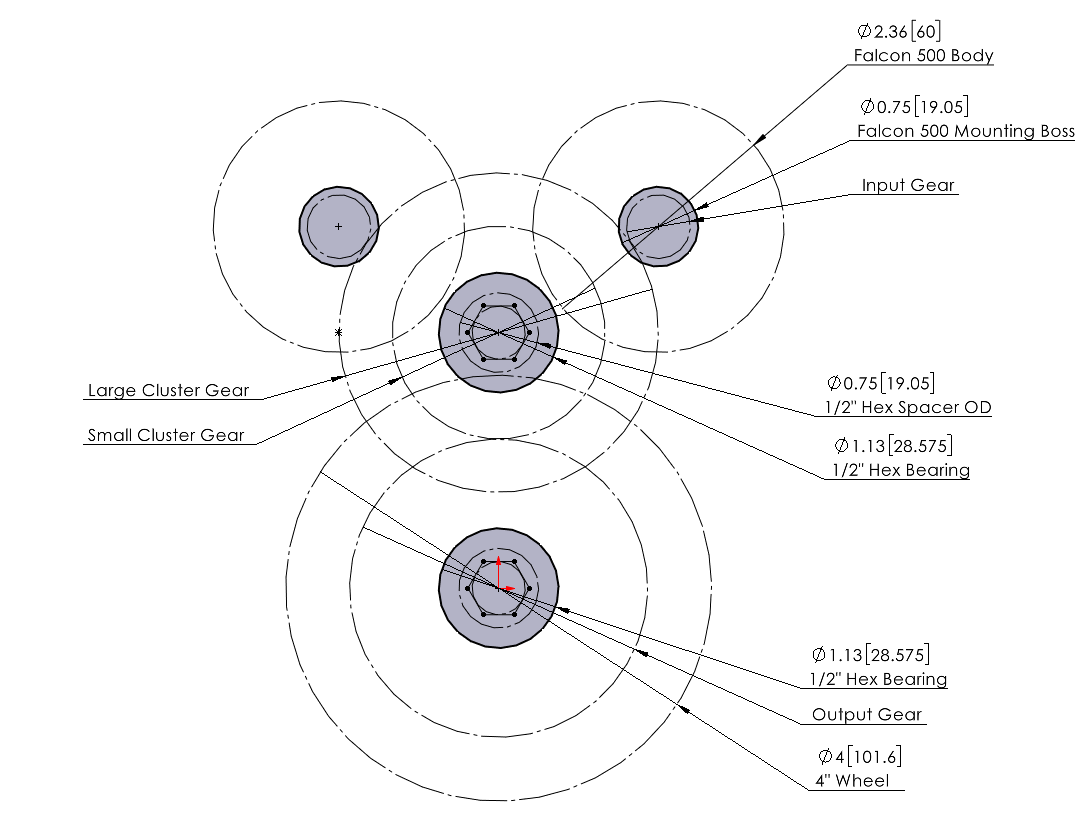
\includegraphics[width=\linewidth]{gearbox_options_layout}
	\end{figure}

	Firstly, we will enter the total ratio of 7:1 and we will allow for up to 1\% deviation from there. For this example we choose to only use gears from Vex, so we uncheck the AndyMark and REV source options.\\
	
	Since our motor input is a Falcon 500, we will change the input gear type to "Falcon Gear". We want the motor gear to be able to fit through the mounting boss hole so the motor can be easily removed, so will will specify that its outer diameter should be less than 0.75".\\
	
	In our gearbox, the cluster gear bearing sticks out the same side of the plate as the motors, so we want to make sure they will not interfere with each other. The motor body's diameter is 2.36", and the bearing's is 1.125". So the minimum distance between their centers without interference is $ \frac{1}{2} \left( 2.36+1.125 \right) \approx 1.75 $". That will be our minimum C-C distance between the input and large cluster gears.\\
	
	Since the motor here sits outside the gearbox, we do not need to worry about it interfering with the small cluster gear (as we would if the gearbox were "flipped" and the motors were inside), so we do not need to set Axle 1 clearance. However, the output shaft goes through the gearbox underneath the large cluster gear, so we must make sure they do not interfere with each other. If the axle were empty underneath the large cluster gear we could set the Axle 4 clearance to "Bore Diam." to let it be automatically selected based on the bore of the output gear. In this case though, we will put a hex spacer with an outer diameter of 0.75", so we will set that as our Axle 4 clearance.\\
	
	We want to make sure that the output gear is smaller than the wheel diameter so that the gear does not hit the ground. To give some margin of safety for a 4" wheel, we will set its maximum diameter at 3.5". In order to limit the size of the gearbox, we will also limit the large cluster gear to have less than 60 teeth.\\
	
	With all of these values input, the calculator looks like this:
	
	\begin{figure}[H]
		\centering
		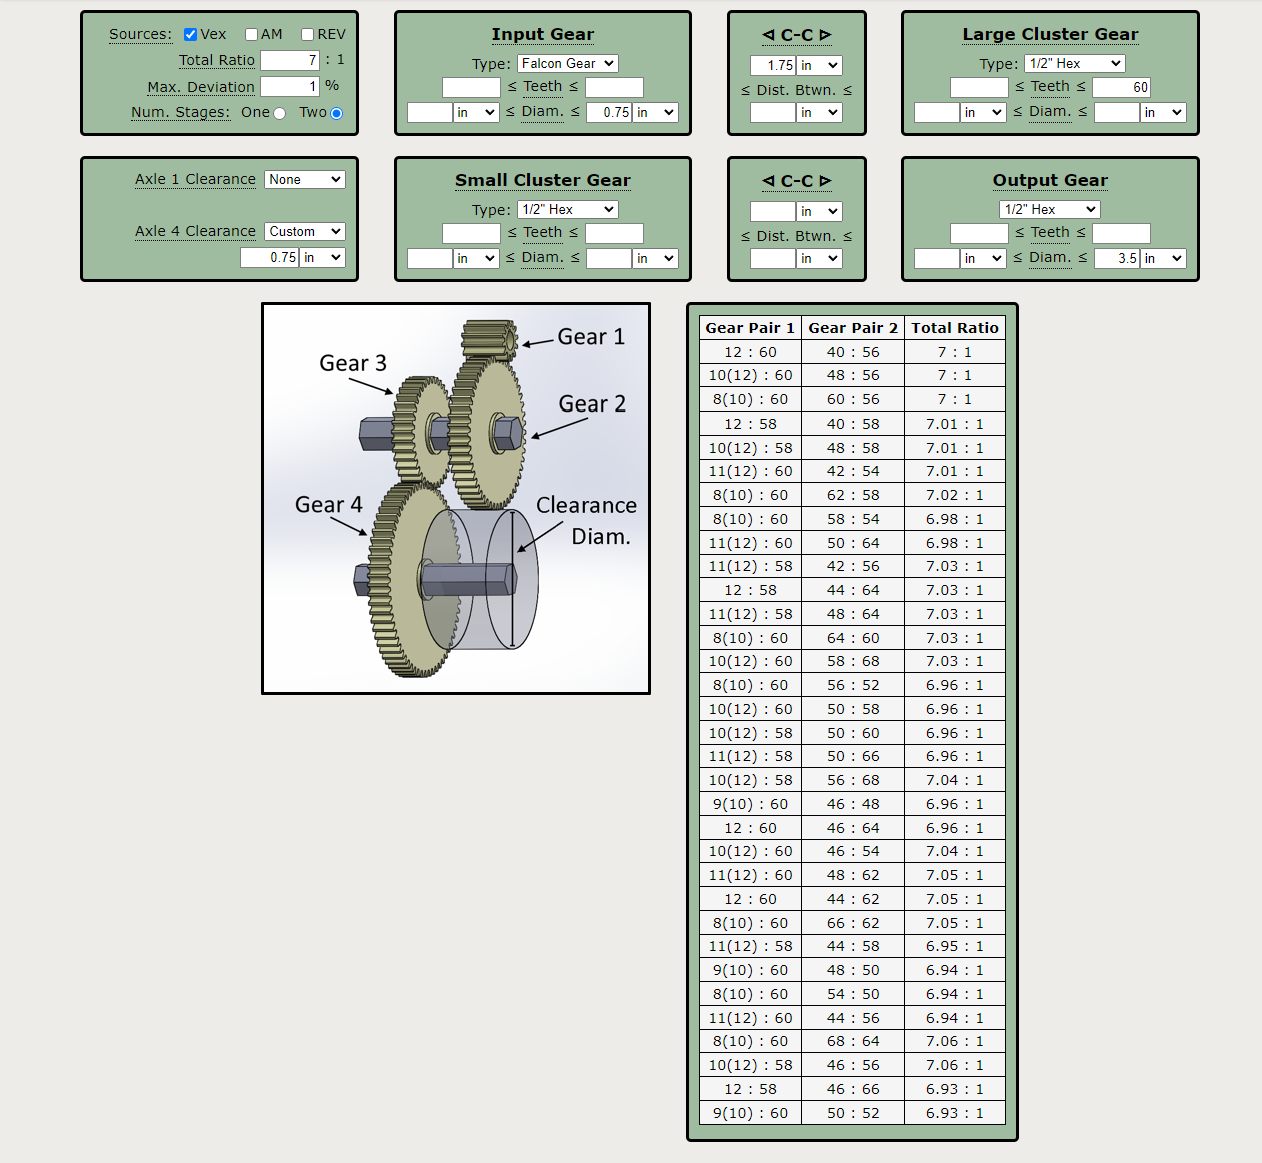
\includegraphics[width=0.9\linewidth]{gearbox_options_screenshot}
	\end{figure}
	
	We can see there are 33 combinations of gears that meet the criteria we set. These are sorted first by deviation from the desired ratio, then by total size. In this case we find the best gearbox suggested has a 12t input gear, 60t large cluster gear, 40t small cluster gear, and 56t output gear.
	
	
	
\end{document}